
\section{\BookRecordIndex{T0047}Seidel 表示}\label{sec:12-5}

设 $(M,\omega)$ 是满足强\BookRecordIndex{T0058}半正性条件~\eqref{eq:8-5-1} 的闭\BookRecordIndex{T0358}辛流形，并设
$\psi=\{\psi_t\}_{t\in\mathbb R/\mathbb Z}$ 是 $M$ 的一条\BookRecordIndex{T0161}哈密顿辛微分同胚环路；它由
哈密顿函数
\[
  \mathbb R/\mathbb Z\times M\longrightarrow\mathbb R,
  \qquad(t,x)\longmapsto K_t(x)
\]
通过
\begin{equation}\label{eq:12-5-1}
  \partial_t\psi_t=Y_t\circ\psi_t,
  \qquad \iota(Y_t)\omega=dK_t
\end{equation}
生成。下文将看到，这样的环路自然作用在弗洛尔\BookRecordIndex{T0246}模空间上。不过，要把它提升为弗洛尔
上链复形上的作用，还须选取一种归一化，也就是\BookRecordIndex{T0156}哈密顿纤维化
$\widetilde M_\psi\to S^2$ 的一个截面同伦类 $\tau$。回忆式~\eqref{eq:8-2-6} 及
定理~\ref{thm:11-4-6} 的证明：$\widetilde M_\psi$ 的截面可以由一对光滑映射
$u_\pm:\mathbb C\to M$ 表示，它们对每个
$z=e^{2\pi(s+it)}\in\mathbb C\setminus\{0\}$ 满足
\[
  u_+(z)=\psi_t\bigl(u_-(1/z)\bigr).
\]
在同伦意义下，可以选取这个截面使得 $|z|\leq1$ 时 $u_+(z)\equiv x_0$。于是，$u_-$ 在
$\mathbb C$ 中单位圆盘上的限制是光滑函数
\[
  \tau:B:=\{z\in\mathbb C\mid |z|\leq1\}\longrightarrow M,
\]
并满足
\begin{equation}\label{eq:12-5-2}
  \tau(e^{-2\pi it})=\psi_t^{-1}(x_0),
  \qquad t\in\mathbb R.
\end{equation}
现在说明这样的偶对 $(\psi,\tau)$ 如何决定弗洛尔上同调的一个同构。

这个同构来自弗洛尔方程~\eqref{eq:12-1-3} 的自然性。设 $(H,J)$ 是
命题~\ref{prop:12-1-2} 中的正则偶对，不过现在允许 $J=J_t$ 依赖于 $t$。令
$u:\mathbb R^2\to M$ 是弗洛尔方程
\[
  \partial_su+J_t(u)\bigl(\partial_tu-X_t(u)\bigr)=0
\]
的一个解，其中 $\iota(X_t)\omega=dH_t$，并定义
\[
  v(s,t):=\psi_t^{-1}\bigl(u(s,t)\bigr).
\]
那么 $v$ 是偶对 $(\psi^*H,\psi^*J)$ 的弗洛尔方程之解，这个偶对定义为
\begin{equation}\label{eq:12-5-3}
  (\psi^*H)_t:=(H_t-K_t)\circ\psi_t,
  \qquad
  (\psi^*J)_t:=\psi_t^*J_t.
\end{equation}
此外，当 $s\to\pm\infty$ 时，$v$ 的极限是 $\psi^*H$ 的（可缩）周期轨道。从构造立即
可见，偶对 $(\psi^*H,\psi^*J)$ 满足与 $(H,J)$ 相同的\BookRecordIndex{T0408}正则性假设。因此，沿 $\psi$ 拉回
给出偶对 $(H,J)$ 与 $(\psi^*H,\psi^*J)$ 的\BookRecordIndex{T0131}弗洛尔连接轨道之间的显然一一对应，进而给出
相应 $1$-周期轨道集之间的一一对应。后一个对应是映射
\[
  \mathcal P_0(H)\longrightarrow\mathcal P_0(\psi^*H),
  \qquad x\longmapsto\psi^*x,
\]
其中
\[
  \psi^*x(t):=\psi_t^{-1}(x(t)),
  \qquad t\in\mathbb R.
\]

为了得到弗洛尔上同调的同构，必须选取一个双射
\[
  \widetilde{\mathcal P}(H)\longrightarrow
  \widetilde{\mathcal P}(\psi^*H),
\]
使它下降为双射 $\mathcal P_0(H)\to\mathcal P_0(\psi^*H)$，并且关于 $H_2^S(M)$ 的
作用等变。这样的双射有许多个，每一个都给出一个弗洛尔上同调同构；截面 $\tau$ 则提供
一个典范选择。为看清这一点，注意每个 $\widetilde x\in\widetilde{\mathcal P}(H)$ 都可
由偶对 $(x,u)$ 表示，并使得 $|z|\leq1/2$ 时 $u(z)=x_0$。定义
\[
  (\psi,\tau)^*\widetilde x
  \in\widetilde{\mathcal P}(\psi^*H)
  \sourcefootnote{原书把这里的陪域印作尚未定义的
  $\widetilde{\mathcal P}(H^\alpha)$；同页前后的双射与映射均明确给出陪域
  $\widetilde{\mathcal P}(\psi^*H)$，故据此补正。}
\]
为
\[
  (\psi,\tau)^*\widetilde x
  :=\bigl(\psi^*x,(\psi,\tau)^*u\bigr),
\]
其中
\[
  ((\psi,\tau)^*u)(re^{2\pi it}):=
  \begin{cases}
    \psi_t^{-1}\bigl(u(re^{2\pi it})\bigr),&1/2\leq r\leq1,\\
    \tau(2re^{-2\pi it}),&0\leq r\leq1/2.
  \end{cases}
\]
注意，映射
\[
  \widetilde{\mathcal P}(H)\longrightarrow
  \widetilde{\mathcal P}(\psi^*H),
  \qquad
  \widetilde x\longmapsto(\psi,\tau)^*\widetilde x
\]
关于 $H_2^S(M)$ 的作用等变。

\begin{exercise}\label{ex:12-5-1}
证明：对 $A\in H_2^S(M)$，有
\[
  (\psi,\tau)^*(A\#\widetilde x)
  =(\psi,\tau-\iota_*A)^*\widetilde x,
\]
并且
\[
  \mu_{\mathrm{CZ}}\bigl((\psi,\tau)^*\widetilde x\bigr)
  =\mu_{\mathrm{CZ}}(\widetilde x)+2c(\tau),
  \qquad
  \mathcal A_{\psi^*H}\bigl((\psi,\tau)^*\widetilde x\bigr)
  =\mathcal A_H(\widetilde x)+\widetilde\omega_\psi(\tau).
\]
这里
\[
  c:=c_1^{\mathrm{Vert}}\in H^2(\widetilde M_\psi)
\]
表示竖直第一 Chern 类，而
$\widetilde\omega_\psi\in\Omega^2(\widetilde M_\psi)$ 是一个\BookRecordIndex{T0155}哈密顿联络的\BookRecordIndex{T0260}耦合形式。
\end{exercise}

弗洛尔上链复形之间有一个同构
\[
  \mathcal S(\psi,\tau;H):
  \operatorname{CF}^*(H)\longrightarrow\operatorname{CF}^*(\psi^*H),
\]
定义为
\[
  \bigl(\mathcal S(\psi,\tau;H)\xi\bigr)
  \bigl((\psi,\tau)^*\widetilde x\bigr):=\xi(\widetilde x),
\]
其中 $\xi\in\operatorname{CF}^*(H)$、
$\widetilde x\in\widetilde{\mathcal P}(H)$。只要 $(H,J)$ 是命题~\ref{prop:12-1-2}
中的正则偶对，它就在弗洛尔上同调上诱导一个同构
\[
  \mathcal S(\psi,\tau;H,J):
  \operatorname{HF}^*(H,J)
  \longrightarrow
  \operatorname{HF}^*(\psi^*H,\psi^*J).
\]
所需的自同构
\[
  \mathcal S^{H,J}(\psi,\tau):
  \operatorname{HF}^*(H,J)\longrightarrow\operatorname{HF}^*(H,J)
\]
是同构 $\mathcal S(\psi,\tau;H,J)$（可以把它看作一次“扭曲”）与
定理~\ref{thm:12-1-3} 的延拓同构
\[
  \operatorname{HF}^*(\psi^*H,\psi^*J)
  \longrightarrow\operatorname{HF}^*(H,J)
\]
的复合。

沿用第~\ref{sec:12-1} 节的记号，简写
$\mathcal S^\alpha:=\mathcal S^{H^\alpha,J^\alpha}$。从构造显然可见，Seidel 同态关于
定理~\ref{thm:12-1-3} 的延拓同构是自然的，即
\[
  \mathcal S^\beta(\psi,\tau)\circ\Phi^{\beta\alpha}
  =\Phi^{\beta\alpha}\circ\mathcal S^\alpha(\psi,\tau)
\]
对所有 $\alpha,\beta$ 都成立；而且这确实是一个表示，也就是说
\[
  \mathcal S^\alpha(\phi,\sigma)\circ\mathcal S^\alpha(\psi,\tau)
  =\mathcal S^\alpha(\phi\psi,\sigma\#\tau)
\]
对任意两条哈密顿环路 $\phi,\psi$ 及其相应截面 $\sigma,\tau$ 都成立。我们把两个截面的
\BookRecordIndex{T0227}连通和 $\sigma\#\tau$ 的确切含义留给读者写出。关于这个运算，偶对 $(\phi,\sigma)$ 的
同伦类构成一个群 $\widetilde G$；它是
$G:=\pi_1(\operatorname{Ham}(M,\omega))$ 被环路空间 $\mathcal L M$ 的甲板变换群
$H_2^S(M)$ 扩张所得的群。\footnote{这里应把 $H_2^S(M)$ 理解为 Hurewicz 同态在无挠群
$H_2(M;\mathbb Z)/\operatorname{tor}$ 中的像；见注~\ref{rem:12-5-4}。}
赋值
\[
  (\phi,\sigma)\longmapsto\mathcal S^{H,J}(\phi,\sigma)
\]
定义了 $\widetilde G$ 在弗洛尔上同调这个 $\Lambda$-模的同构空间上的表示。Seidel 证明，
这些同构 $\mathcal S(\phi,\sigma)$ 保持
$\operatorname{HF}^*(H,J)$ 的右 $\operatorname{HF}^*(H,J)$-模结构，即
\[
  \mathcal S^{H,J}(\phi,\sigma)(a*b)
  =\bigl(\mathcal S^{H,J}(\phi,\sigma)a\bigr)*b
\]
对所有 $a,b\in\operatorname{HF}^*(H,J)$ 成立。从这个观点看，困难之处是证明弗洛尔
上同调上的 \BookRecordIndex{T0047}Seidel 表示，在定理~\ref{thm:12-1-4} 的同构下与\BookRecordIndex{T0229}量子上同调上的 \BookRecordIndex{T0047}Seidel 表示
一致。这正是下面定理的内容。

\begin{theorem}[Seidel]\label{thm:12-5-2}
设 $(M,\omega)$ 满足~\eqref{eq:8-5-1}。那么，对每个正则偶对
$(H^\alpha,J^\alpha)$、每条哈密顿环路 $\psi$ 以及每个相应截面 $\tau$，都有
\[
  \mathcal S(\psi,\tau)*(\Phi^\alpha\xi^\alpha)
  =\Phi^\alpha\bigl(\mathcal S^\alpha(\psi,\tau)\xi^\alpha\bigr)
\]
对每个 $\xi^\alpha\in\operatorname{HF}^*(H^\alpha,J^\alpha)$ 成立。这里
\[
  \Phi^\alpha:
  \operatorname{HF}^*(H^\alpha,J^\alpha)
  \longrightarrow\operatorname{QH}^*(M;\Lambda_\omega)
\]
是定理~\ref{thm:12-1-4} 的 PSS 同构，而
$\mathcal S(\psi,\tau)\in\operatorname{QH}^*(M;\Lambda_\omega)$ 是
第~\ref{sec:11-4} 节定义的 \BookRecordIndex{T0046}Seidel 元。
\end{theorem}

定理~\ref{thm:12-5-2} 的证明运用了注~\ref{rem:12-1-7} 中描述的思想。Seidel 同态
$\mathcal S^\alpha(\psi,\tau)$
\sourcefootnote{原书在这里把 $\mathcal S^\alpha(\psi,\tau)$ 称为 \BookRecordIndex{T0046}Seidel 元；但前文已将它
定义为弗洛尔上同调上的 Seidel 同态，而本定理中的量子 \BookRecordIndex{T0046}Seidel 元是不带 $\alpha$ 的
$\mathcal S(\psi,\tau)$，故据此改正对象名称。}
计数依赖于 $s$ 的弗洛尔方程之解，而 $\Phi^\alpha$ 计数\BookRecordIndex{T0182}尖盘。通过把两个\BookRecordIndex{T0182}尖盘
粘到一个弗洛尔圆柱的两端，可以得到定理~\ref{thm:12-5-2} 的关系；这样便构造出\BookRecordIndex{T0156}哈密顿
纤维化 $\widetilde M_\psi\to S^2$ 的一个 $J$-全纯截面。细节见 Seidel 
\srcite{363}。

\begin{lemma}\label{lem:12-5-3}
设
\[
  \mathbb R/\mathbb Z\longrightarrow\operatorname{Ham}(M,\omega),
  \qquad t\longmapsto\psi_t
\]
是满足 $\psi_0=\operatorname{id}$ 的一条\BookRecordIndex{T0161}哈密顿辛微分同胚环路，$\tau$ 是
$\widetilde M_\psi$ 的一个截面同伦类。设
$\widetilde\phi\in\widetilde{\operatorname{Ham}}(M,\omega)$ 是一条满足
$\phi_0=\operatorname{id}$ 的道路
\[
  [0,1]\longrightarrow\operatorname{Ham}(M,\omega),
  \qquad t\longmapsto\phi_t,
\]
的等价类。那么，对每个
$a\in\operatorname{QH}^*(M;\Lambda_\omega)$，都有
\[
  \rho(\psi^*\widetilde\phi;a)
  =\rho\bigl(\widetilde\phi;\mathcal S(\psi,\tau)a\bigr)
   +\widetilde\omega_\psi(\tau),
\]
其中 $\psi^*\widetilde\phi$ 表示道路
$t\mapsto\psi_t^{-1}\circ\phi_t$ 的等价类。
\end{lemma}

\begin{proof}
使用习题~\ref{ex:12-4-7} 中\BookRecordIndex{T0271}谱不变量的上同调描述。固定一个生成
$\widetilde\phi$ 的哈密顿函数
$H:\mathbb R/\mathbb Z\times M\to\mathbb R$。按构造，上面得到的同态
\[
  \mathcal S(\psi,\tau;H,J):
  \operatorname{HF}^*(H,J)
  \longrightarrow
  \operatorname{HF}^*(\psi^*H,\psi^*J)
\]
把 $\operatorname{HF}_\kappa^*(H,J)$ 同构地映到
$\operatorname{HF}_{\kappa+\widetilde\omega_\psi(\tau)}^*
(\psi^*H,\psi^*J)$。所以有交换图
\[
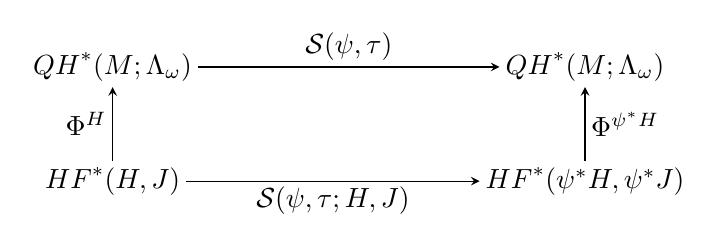
\begin{tikzpicture}[baseline=(current bounding box.center),>=stealth,
  every node/.style={inner sep=2pt}]
  \node (q1) at (0,1.45) {$\operatorname{QH}^*(M;\Lambda_\omega)$};
  \node (q2) at (6.0,1.45) {$\operatorname{QH}^*(M;\Lambda_\omega)$};
  \node (h1) at (0,0) {$\operatorname{HF}^*(H,J)$};
  \node (h2) at (6.0,0) {$\operatorname{HF}^*(\psi^*H,\psi^*J)$};
  \draw[->] (q1) -- node[above] {$\mathcal S(\psi,\tau)$} (q2);
  \draw[->] (h1) -- node[below] {$\mathcal S(\psi,\tau;H,J)$} (h2);
  \draw[->] (h1) -- node[left] {$\Phi^H$} (q1);
  \draw[->] (h2) -- node[right] {$\Phi^{\psi^*H}$} (q2);
\end{tikzpicture}
\]
其中上方水平箭头把 $j_\kappa(H)$ 的像同构地映到
$j_{\kappa+\widetilde\omega_\psi(\tau)}(\psi^*H)$ 的像。

现在令 $\kappa\in\mathbb R\setminus\operatorname{Spec}(H)$。由
习题~\ref{ex:12-5-1}，有
$\kappa+\widetilde\omega_\psi(\tau)\notin\operatorname{Spec}(\psi^*H)$。此外，由
习题~\ref{ex:12-4-7}，
\[
\begin{aligned}
  \kappa<-\rho(\widetilde\phi^{-1};a)
  &\quad\Longleftrightarrow\quad
  a\in\operatorname{im}j_\kappa(H)\\
  &\quad\Longleftrightarrow\quad
  \mathcal S(\psi,\tau)a
  \in\operatorname{im}j_{\kappa+\widetilde\omega_\psi(\tau)}(\psi^*H)\\
  &\quad\Longleftrightarrow\quad
  \kappa+\widetilde\omega_\psi(\tau)
  <-\rho\bigl((\psi^*\widetilde\phi)^{-1};
  \mathcal S(\psi,\tau)a\bigr).
\end{aligned}
\]
第二个等价关系来自上面的交换图，最后一个等价关系再次来自
习题~\ref{ex:12-4-7}。因此
\[
  \rho(\widetilde\phi^{-1};a)
  =\rho\bigl((\psi^*\widetilde\phi)^{-1};
  \mathcal S(\psi,\tau)a\bigr)
   +\widetilde\omega_\psi(\tau).
\]
把道路 $t\mapsto\phi_t$ 换成 $t\mapsto\phi_t^{-1}\circ\psi_t$，即得所断言的公式。
\end{proof}

Oh \srcite{306} 把 Seidel 作用下\BookRecordIndex{T0271}谱不变量的平移称为\emph{\BookRecordIndex{T0096}单值化平移}。使用系数环
\[
  \Lambda:=\Lambda^{\mathrm{univ}}[q,q^{-1}]
\]
时，可以通过把 $\tau$ 的选取标准化为 $\widetilde\omega_\psi(\tau)=0$ 来消去\BookRecordIndex{T0096}单值化平移
（见 Lalonde--McDuff--Polterovich \srcite{228}）。即便如此，如果\BookRecordIndex{T0229}量子上同调上的 Seidel
作用对某个流形非平凡，那么\BookRecordIndex{T0271}谱不变量所含信息仍只有不变部分才能下降到
$\operatorname{Ham}(M)$。下文注~\ref{rem:12-5-5} 将作更完整的解释；下一条注先给出
\BookRecordIndex{T0096}单值化平移的整体框架。

\begin{remark}[\BookRecordIndex{T0271}谱不变量：整体观点]\label{rem:12-5-4}
先构造一个以 $\operatorname{Ham}(M,\omega)$ 为底的纤维空间
$P\operatorname{Ham}(M,\omega)$，它的基本群是上面考虑的扩张 $\widetilde G$。为简单起见，
以下假设 $M$ 单连通且 $\pi_2(M)$ 无挠；于是 $\widetilde G$ 是 $G$ 被整个群
\[
  \pi_1(\mathcal L M)\cong\pi_2(M)
\]
扩张所得的群，而不是被其商群 $H_2^S(M)$ 扩张所得的群。

固定基点 $x_0\in M$，以 $P_0M$ 表示从 $\gamma(0)=x_0$ 出发的光滑道路
$\gamma:[0,1]\to M$ 所成的空间。记
\[
  P\operatorname{Ham}(M,\omega)
  \subset\operatorname{Ham}(M,\omega)\times P_0M
\]
为满足 $\gamma(1)=\phi^{-1}(x_0)$ 的偶对 $(\phi,\gamma)$ 所成的空间。有一个\BookRecordIndex{T0279}纤维化
\[
  \Omega M\longrightarrow P\operatorname{Ham}(M,\omega)
  \longrightarrow\operatorname{Ham}(M,\omega),
\]
其纤维是 $M$ 的基环路空间 $\Omega M$。同伦正合列中的\BookRecordIndex{T0063}边界映射
\[
  \pi_2(\operatorname{Ham}(M,\omega))
  \longrightarrow\pi_1(\Omega M)\cong\pi_2(M)
\]
由在基点处求值给出。众所周知，它的像由挠类组成（例如见 \srcite{227}）。所以，对 $M$
的假设蕴含这个映射为零。因而 $\pi_1(P\operatorname{Ham}(M,\omega))$ 是 $G$ 被
$\pi_2(M)$ 扩张所得的群，并且由式~\eqref{eq:12-5-2}，它同构于 $\widetilde G$。具体地，
每个偶对 $(\psi,\tau)$ 通过
\[
  \gamma_t(s):=\tau(se^{-2\pi it})
\]
决定一条环路
\[
  \mathbb R/\mathbb Z\longrightarrow P\operatorname{Ham}(M,\omega),
  \qquad t\longmapsto(\psi_t,\gamma_t),
\]
并由此诱导所需同构
$\widetilde G\to\pi_1(P\operatorname{Ham}(M,\omega))$。

把 $P\operatorname{Ham}(M,\omega)$ 的万有覆盖记作
$\widetilde{P\operatorname{Ham}}(M,\omega)$。它的元素是
$P\operatorname{Ham}(M,\omega)$ 中道路 $(\phi_t,\gamma_t)_{t\in[0,1]}$ 的等价类
$[\widetilde\phi,\widetilde\gamma]$，其中 $\phi_0=\operatorname{id}$，且 $\gamma_0$ 是
常值道路。群 $\widetilde G$ 以甲板变换作用在
$\widetilde{P\operatorname{Ham}}(M,\omega)$ 上：若 $(\psi,\tau)$ 代表
$\widetilde G$ 的一个元素，而 $[\widetilde\phi,\widetilde\gamma]$ 是
$\widetilde{P\operatorname{Ham}}(M,\omega)$ 中的等价类，则
$(\psi,\tau)\cdot[\widetilde\phi,\widetilde\gamma]$ 表示如下道路的等价类：先沿
$\psi,\tau$ 所确定的 $P\operatorname{Ham}(M,\omega)$ 中环路绕行一周，再沿道路
$(\phi_t,\gamma_t)$ 前进。

考察平凡线丛
\[
  \widetilde{P\operatorname{Ham}}(M,\omega)
  \times\operatorname{QH}^*(M;\Lambda)\times\mathbb R
  \longrightarrow
  \widetilde{P\operatorname{Ham}}(M,\omega)
  \times\operatorname{QH}^*(M;\Lambda).
\]
群 $\widetilde G$ 作用在这个线丛上：它在
$\widetilde{P\operatorname{Ham}}(M,\omega)$ 上作甲板变换，在\BookRecordIndex{T0229}量子上同调上作 \BookRecordIndex{T0047}Seidel
表示，在 $\mathbb R$ 上作\BookRecordIndex{T0096}单值化平移。更确切地，
\[
  (\psi,\tau)\cdot
  \bigl([\widetilde\phi,\widetilde\gamma];a;\kappa\bigr)
  =\bigl((\psi,\tau)\cdot[\widetilde\phi,\widetilde\gamma];
  \mathcal S(\psi,\tau)a;
  \kappa+\widetilde\omega_\psi(\tau)\bigr).
\]
引理~\ref{lem:12-5-3} 断言，\BookRecordIndex{T0271}谱不变量定义了这个丛的一个 $\widetilde G$-等变截面
\[
  \rho:
  \widetilde{P\operatorname{Ham}}(M,\omega)
  \times\operatorname{QH}^*(M;\Lambda)
  \longrightarrow
  \widetilde{P\operatorname{Ham}}(M,\omega)
  \times\operatorname{QH}^*(M;\Lambda)\times\mathbb R.
\]
对 $\widetilde G$ 取商后，得到相应实线丛 $L\to X$ 的一个截面；这里 $X$ 是\BookRecordIndex{T0279}纤维化
\[
  \operatorname{QH}^*(M;\Lambda)
  \longrightarrow
  X:=\widetilde{P\operatorname{Ham}}(M,\omega)
  \times_{\widetilde G}\operatorname{QH}^*(M;\Lambda)
  \longrightarrow P\operatorname{Ham}(M)
\]
的总空间。

谱值也有类似图景。由习题~\ref{ex:12-5-1}，$\widetilde G$ 在
$\widetilde{P\operatorname{Ham}}(M,\omega)\times\mathbb R$ 上的作用保持谱值子集
\[
  \mathfrak{spec}:=
  \bigl\{([\widetilde\phi,\widetilde\gamma],c)
  \in\widetilde{P\operatorname{Ham}}(M,\omega)\times\mathbb R
  \bigm|c\in\operatorname{Spec}(\widetilde\phi)\bigr\}.
\]
所以商 $\mathfrak{spec}/\widetilde G$ 是实线丛
\[
  L:=\widetilde{P\operatorname{Ham}}(M,\omega)
  \times_{\widetilde G}\mathbb R
  \longrightarrow P\operatorname{Ham}(M,\omega)
\]
的一个子集。
\end{remark}

\begin{remark}\label{rem:12-5-5}
弗洛尔（上）同调的定义有许多可能变体。下一节将为任意辛微分同胚 $\phi$ 定义精简版本
$\operatorname{HF}^*(\phi)$；作为引入，这里先简述其中两种变体。

\begin{enumerate}[label=(\roman*)]
\item 首先考虑以例~\ref{ex:11-1-4}(vi) 的环
\[
  \Lambda:=\Lambda^{\mathrm{univ}}[q,q^{-1}]
\]
为系数的弗洛尔上同调，其中基环为 $R$。在此情形，对每个正则哈密顿量 $H$，弗洛尔
上链复形 $\operatorname{CF}^*(H;\Lambda)$ 是所有函数
\[
  \xi:\widetilde{\mathcal P}(H)\longrightarrow\Lambda
\]
之集，它们在如下意义下等变：
\begin{equation}\label{eq:12-5-4}
  \xi(A\#\widetilde x)
  =\xi(\widetilde x)t^{\omega(A)}q^{c_1(A)}.
\end{equation}
这对每个 $\widetilde x\in\widetilde{\mathcal P}(H)$ 和每个
$A\in H_2^S(M)$
\sourcefootnote{原书把这里的量词印作 $A\in H_2(M)$；但
$A\#\widetilde x$ 只对第~\ref{sec:12-1} 节定义的甲板变换群 $H_2^S(M)$ 有定义，且本段
前后均使用该群，故补正。}
成立。这是有限生成自由 $\Lambda$-模。元素
$\xi\in\operatorname{CF}^*(H;\Lambda)$ 的次数为 $k$，当且仅当
$\xi(\widetilde x)$ 具有纯次数，并且
\[
  \mu_{\mathrm{CZ}}(\widetilde x)
  +\deg\bigl(\xi(\widetilde x)\bigr)=k
\]
对每个 $\widetilde x\in\widetilde{\mathcal P}(H)$ 成立。弗洛尔上边缘算子仍由
式~\eqref{eq:12-1-9} 定义；容易验证，只要 $\xi$ 满足~\eqref{eq:12-5-4}，
$\delta\xi$ 也满足该式。读者可以验证，$\delta\xi$ 的确是一个定义在
$\widetilde{\mathcal P}(H)$ 上、取值于 $\Lambda$ 的函数。第~\ref{sec:12-1}、
\ref{sec:12-2} 节的全部讨论都适用于这个弗洛尔上同调定义。

现在令 $t\mapsto\psi_t=\psi_{t+1}$ 是一条\BookRecordIndex{T0161}哈密顿辛微分同胚环路，并设哈密顿函数族
$K_t=K_{t+1}:M\to\mathbb R$ 通过式~\eqref{eq:12-5-1} 生成它。固定正则偶对 $(H,J)$，
并由~\eqref{eq:12-5-3} 定义 $(\psi^*H,\psi^*J)$。这条哈密顿环路诱导\BookRecordIndex{T0259}扭曲算子
\[
  \mathcal S(\psi;H,J):
  \operatorname{HF}^*(H,J)
  \longrightarrow\operatorname{HF}^*(\psi^*H,\psi^*J).
\]
在上链\BookRecordIndex{T0072}层次，它定义为
\[
  \bigl(\mathcal S(\psi;H,J)\xi\bigr)
  \bigl((\psi,\tau)^*\widetilde x\bigr)
  :=\xi(\widetilde x)
  t^{-\widetilde\omega_\psi(\tau)}q^{-c(\tau)},
\]
其中 $\xi\in\operatorname{CF}^*(H;\Lambda)$、
$\widetilde x\in\widetilde{\mathcal P}(H)$，而 $\tau$ 是 $\widetilde M_\psi$ 的任意截面。
由习题~\ref{ex:12-5-1} 和式~\eqref{eq:12-5-4}，右端与 $\tau$ 的选择无关。与前面相同，
$\mathcal S(\psi;H,J)$ 下降为弗洛尔上同调上的良定义同构，再经延拓诱导自同构
\[
  \mathcal S^{H,J}(\psi):
  \operatorname{HF}^*(H,J)\longrightarrow\operatorname{HF}^*(H,J).
\]
归根结底，我们得到 $G=\pi_1(\operatorname{Ham}(M,\omega))$ 在弗洛尔上同调上的一个表示。

\item 如果愿意使用模 $2$ 分次，就可以在上述讨论中令 $q=1$；这样得到的弗洛尔上同调群
以\BookRecordIndex{T0270}普适 Novikov 环 $\Lambda^{\mathrm{univ}}$ 为系数，并带模 $2$ 分次。此时弗洛尔上链复形
是所有满足
\[
  \xi(A\#\widetilde x)=\xi(\widetilde x)t^{\omega(A)}
\]
的函数 $\xi:\widetilde{\mathcal P}(H)\to\Lambda^{\mathrm{univ}}$ 所成的集合。这意味着映射
\[
  \widetilde x\longmapsto
  \xi(\widetilde x)t^{\mathcal A_H(\widetilde x)}
\]
在 $H_2^S(M)$ 的作用下不变，因而下降为从 $\mathcal P_0(H)$ 到
$\Lambda^{\mathrm{univ}}$ 的映射。所以弗洛尔上链复形是 $\Lambda^{\mathrm{univ}}$-模
\[
  \operatorname{CF}^*(H):=
  \operatorname{CF}^*(H;\Lambda^{\mathrm{univ}})
  =\operatorname{Map}\bigl(\mathcal P_0(H),\Lambda^{\mathrm{univ}}\bigr),
\]
而弗洛尔上边缘为
\[
  (\delta\xi)(x):=
  \sum_y\sum_\varepsilon n_\varepsilon(x,y)\xi(y)t^\varepsilon.
\]
这里 $n_\varepsilon(x,y)$ 表示能量 $E(u)=\varepsilon$、从 $x$ 到 $y$ 的指标为一的\BookRecordIndex{T0131}弗洛尔
连接轨道之带符号数。现在 \BookRecordIndex{T0047}Seidel 表示由
\[
  \bigl(\mathcal S(\psi;H)\xi\bigr)(\psi^*x):=\xi(x)
\]
给出，其中 $x\in\mathcal P_0(H)$、$\xi\in\operatorname{CF}^*(H)$。

事实表明，这个复形不保留生成哈密顿量 $H$ 的任何本质信息，完全可以只用时间一映射
$\phi\in\operatorname{Ham}(M,\omega)$ 来定义。不过，若这样做，则从
$\operatorname{HF}^*(\phi_0)$ 到 $\operatorname{HF}^*(\phi_1)$ 的\BookRecordIndex{T0133}弗洛尔延拓映射，一般
依赖于定义它的道路 $\phi_s$ 的同伦类。（这一依赖恰由 \BookRecordIndex{T0047}Seidel 表示度量。）此外，即使
$\phi$ 不是哈密顿的，这个定义仍然成立。于是我们自然走向下一节所讨论的、基础宽广得多的
弗洛尔理论。
\end{enumerate}
\end{remark}
